\chapter[System Evaluation]{Chapter 5: System Evaluation}\label{chap:before_last}
%########################################################
\section{Design Outcomes}\label{sec:DO_}
%########################################################
The design review, constrained by the timing of PCB and component procurement and subsequent prototyping, served primarily as a reference for future enhancements rather than immediate project revisions, aligning with the limitations outlined in the \hyperref[sec:drawbacks]{Hypotheses \& Potential Drawbacks} section. The prototype and debugging phases surfaced several design outcomes, including both the successful implementation of subsystem designs and an identified critical flaw: the malfunction of the UART communication between cell monitoring modules.\newline\newline
\noindent
The communication issue originated from the complex hardware interactions within the Arduino Beetle (DFR0282) microcontrollers, particularly affecting the hybrid daisy-chain serial communication setup. The challenges included maintaining a stable 16 MHz clock for precise UART timing, implementing effective flow control, and ensuring accurate pin configuration. These factors, both individually and collectively, compromised the UART system, as further detailed through exhaustive debugging and analysis.\newline\newline
\noindent
Despite this setback, the communication hardware was independently verified as functional, isolating the issue to the microcontrollers used. All other systems and subsystems performed optimally and will be discussed in this chapter. Chapter \ref{chap:last} will propose future actions for multi-module communication and alternative microcontroller recommendations for the cell monitoring boards.
%########################################################
\section{Valuation Prospect}\label{sec:prospect}
%########################################################
This chapter presents a thorough evaluation of the designed modular Battery Management System, ensuring subsystem compliance with key performance and safety standards. We will conduct exhaustive testing of each subsystem in simulated operational environments to verify performance within optimal thresholds. Tests include electrical, thermal, and fault response assessments to establish reliability, state-of-charge accuracy, and overall system integrity. Additionally, we will analyze performance under variable load conditions to evaluate module adaptability and robustness. Our systematic evaluation aims to provide a detailed understanding of subsystem operation and integration within the BMS, guaranteeing cohesive operation, battery longevity, and user safety upon final assembly. This strategy underpins the BMS's integrative success by confirming the efficacy of individual subsystems.\newpage
%########################################################
\section{Prototyping}\label{sec:theProto}
%########################################################
\begin{figure}[h!]
\centering
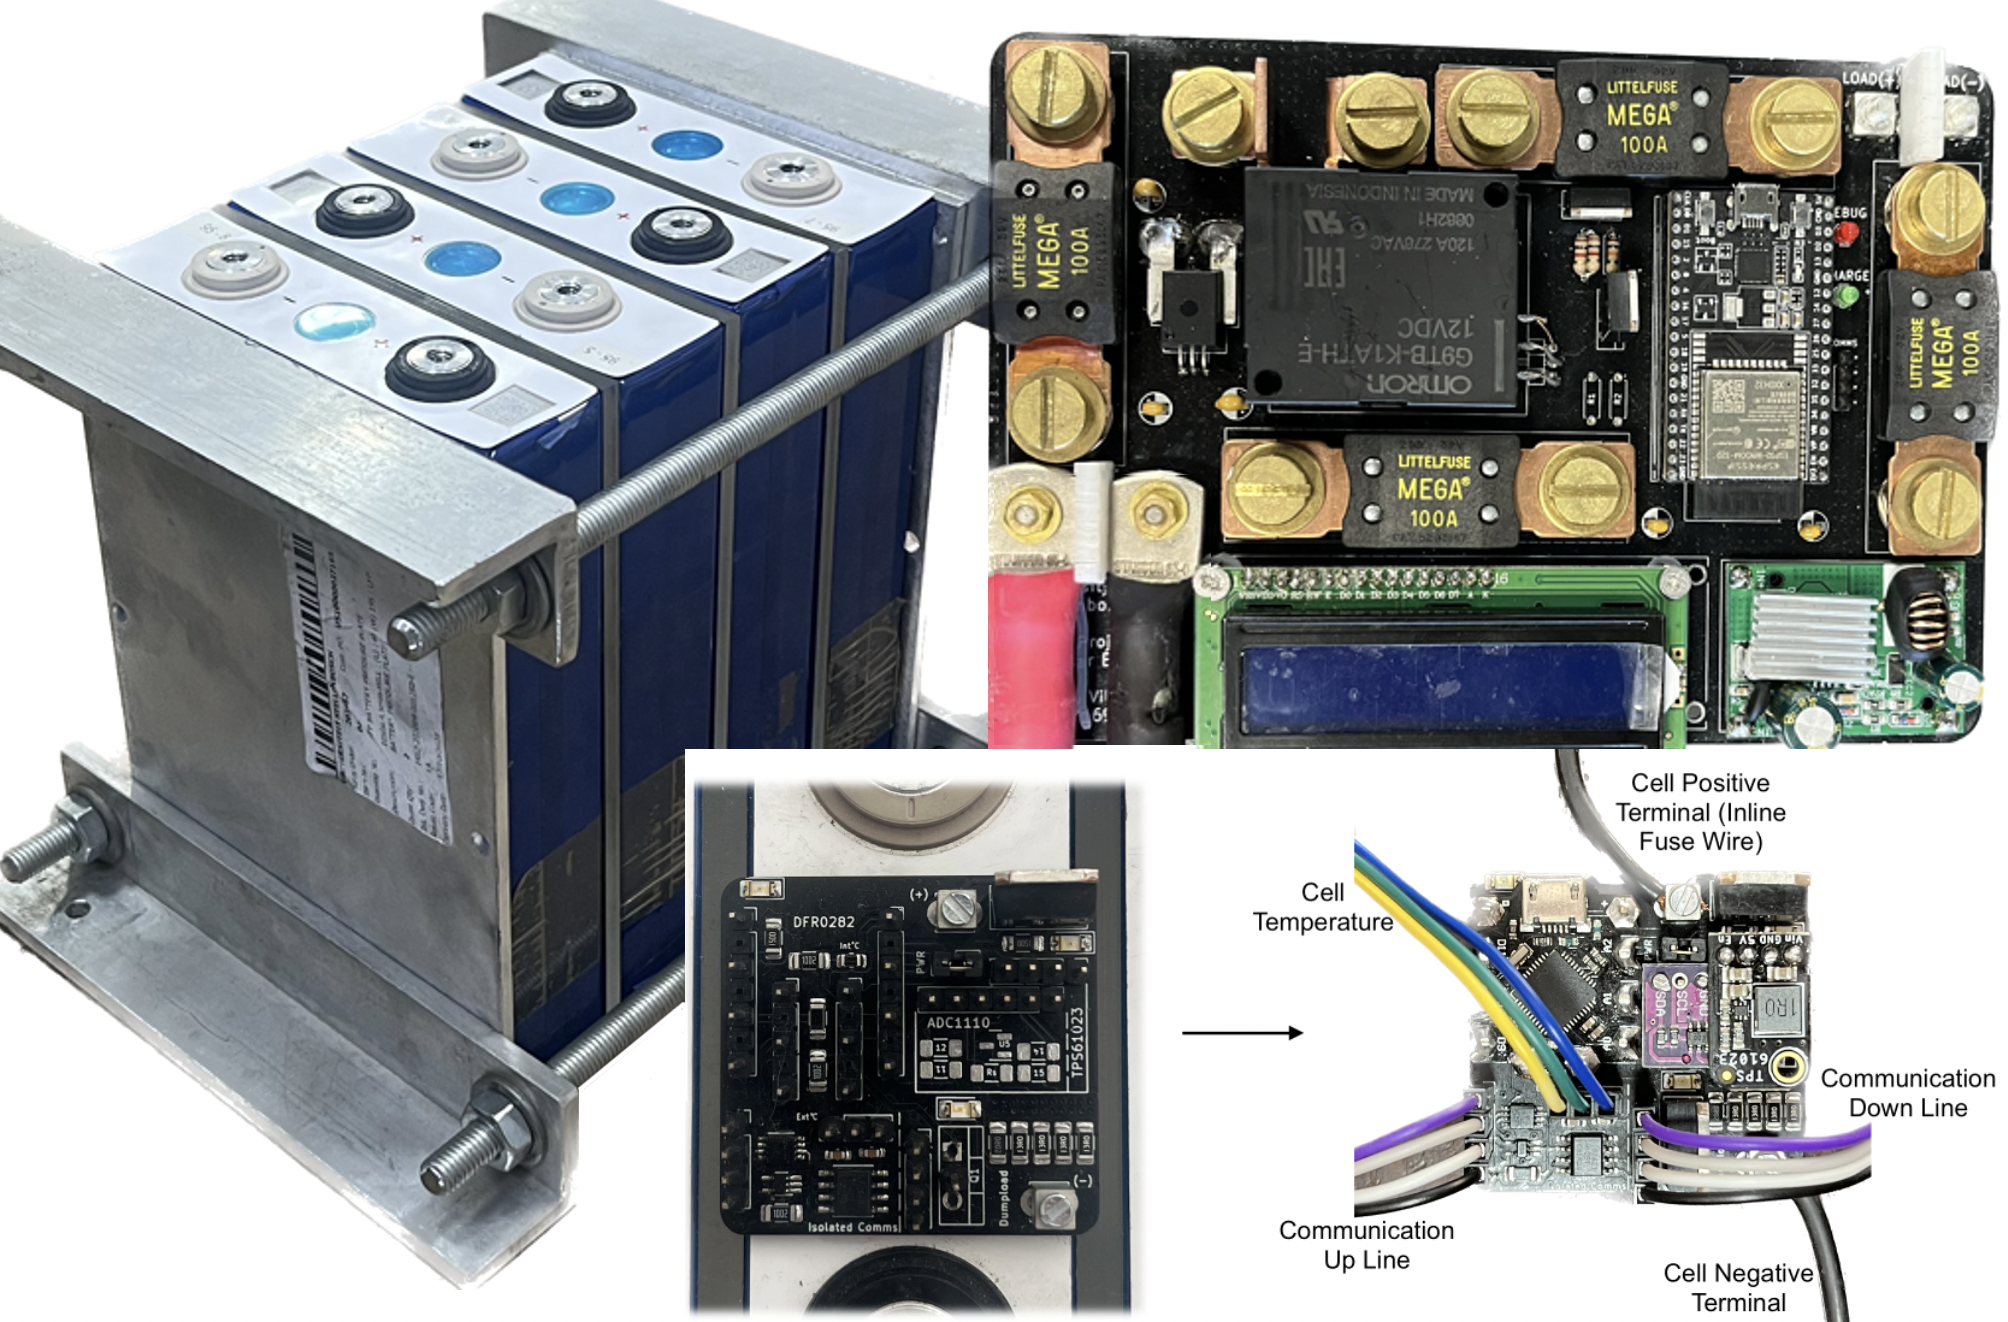
\includegraphics[width=1.0\textwidth]{Skripsie_LaTeXTemplate/Figures/proton.png}
\caption{Design \& Evaluation Prototype Builds}
\label{fig:protonn}
\end{figure}

\noindent
The provided figures showcase a constructed battery pack for experimental testing (left), an engineered main controller (top right), and a cell monitoring module prototype (bottom right). The assembly uses 100Ah 3.2V LFP cells, secured by corner profiles, threaded rods, and aluminium end plates, which, along with Perspex spacers, enforce cell compression to mitigate expansion and maintain cell integrity during discharge cycles. This technique safeguards against delamination from mechanical stress, essential for LFP cell performance. The main controller is optimized for current handling, while the monitoring modules focus on precision and compact design, serving to assess the performance of the Modular BMS systems in the project.
%########################################################
\section{Performance analysis}\label{sec:systEVAL}
%########################################################
This section elaborates on the experimental procedures conducted to assess the performance of the engineered system and its component subsystems under controlled conditions. It encompasses a description of individual tests and includes accompanying subsections that present flow diagrams, result graphs, and model configurations for a comprehensive analysis.\newpage
%*******************************************%
\subsubsection{General}\label{subsec:genZ}
%*******************************************%
The master controller and cell monitoring modules were assessed for functionality using flag-based test programs, which confirmed the onboard Debug LED system operated as intended. Calibration of the NTC sensor on the cell monitoring modules was achieved by referencing an external digital temperature sensor for internal temperature measurements. Validation of these measurements was conducted against the precise readings from a Fluke TiS20 thermal tool. Additionally, an emergency restart test was successfully executed on the cell monitoring module by transmitting a UART force reset flag, causing a momentary power loss in the microcontroller before a successful reboot.
%*******************************************%
\subsubsection{Communication Circuitry}\label{subsec:CCT}
%*******************************************%
The isolated communication system was tested utilizing an ESP32 microcontroller, wherein four GPIO pins were configured as digital outputs to simulate UART transmission (TX) for distinct cell monitoring modules. Correspondingly, four digital input pins on the ESP32 were employed to represent the reception (RX) points within the communication network, ensuring bi-directional connectivity between the microcontroller and each monitoring module's communication subsystem.

\begin{figure}[h!]
\centering
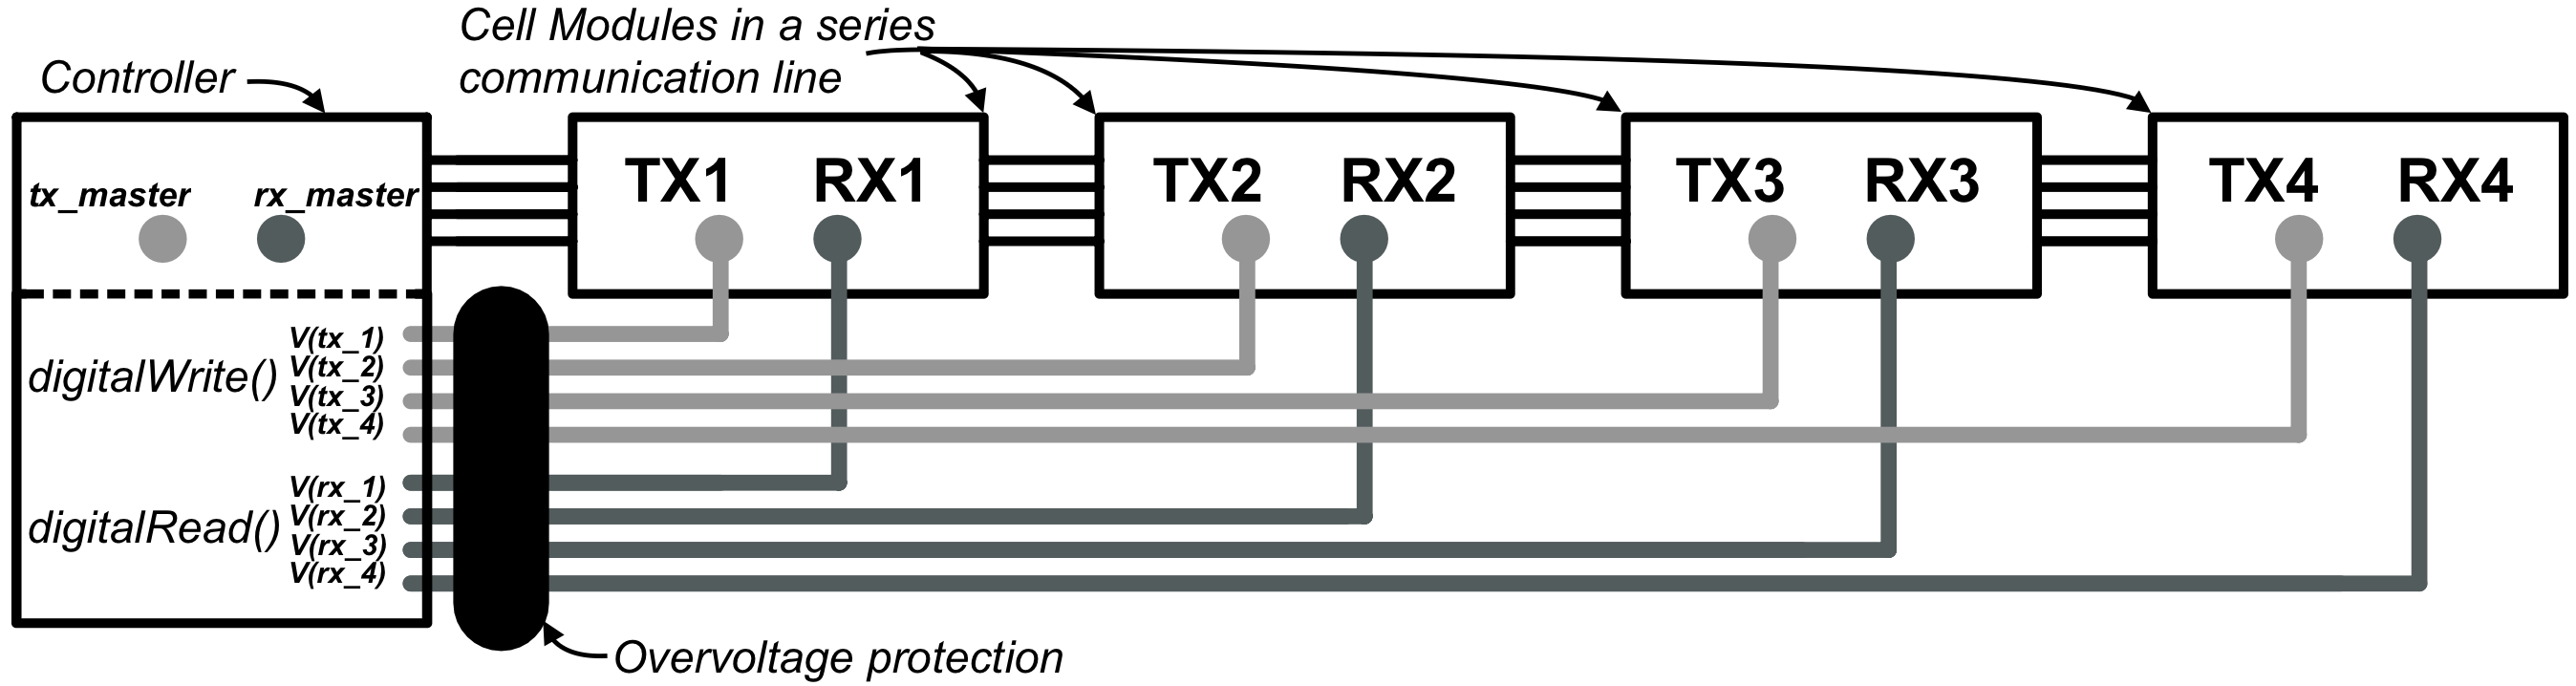
\includegraphics[width=0.75\textwidth]{Skripsie_LaTeXTemplate/Figures/theCOMMStest.png}
\caption{Communication System Test Setup}
\label{fig:comsEXP1}
\end{figure}
\noindent
Figure \ref{fig:comsEXP2} on the next page displays a serial plotter graphing both transmitted and received pulse signals. Over-voltage protection modules safeguarded the ESP32's GPIO pins, with a threshold set slightly above 5V, to mitigate bus contention risks, which didn't occur. Thus, the monitoring modules' communication circuitry operated effectively, incorporating protection logic gates that successfully prevented bus contention. This was confirmed during tests where simultaneous pulsing of two transmit pins (tx2 and tx3) occurred between 40ms and 70ms, with the received signal voltage capped at 5V. This scenario resulted in message corruption but precluded hardware damage, demonstrating the isolated communication system's resilience to potential malfunctions.\newline\newline
\noindent
It is important to note that the logic gates also serves the purpose of eliminating transmission-echo in the communication system, as we can see on the graphs now RX receives a signal transmitted from its corresponding TX. Overall, the communication circuitry integrated into each cell monitoring module functioned as expected.
\newpage
\begin{figure}[h!]
\centering
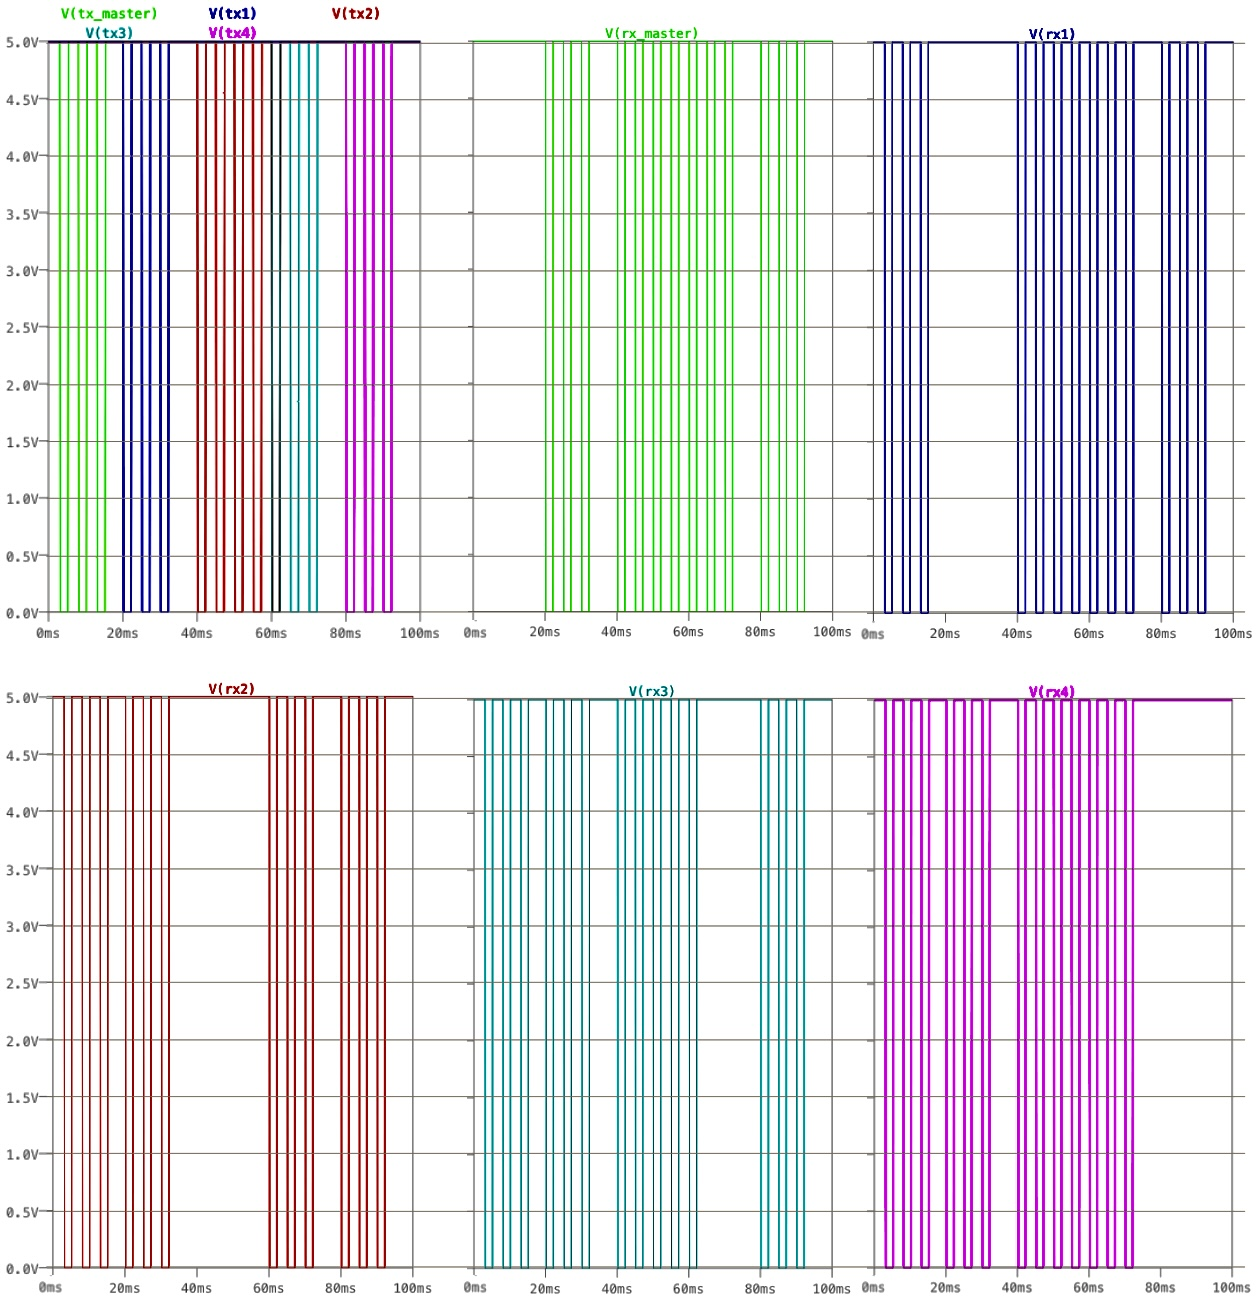
\includegraphics[width=0.72\textwidth]{Skripsie_LaTeXTemplate/Figures/theCOMMStestRES.jpg}
\caption{UART Representative Logic Pulses Measured by ESP32}
\label{fig:comsEXP2}
\end{figure}
%*******************************************%
\subsubsection{UART, Voltage measurement \& Cell Balancing}\label{subsec:CBT}
%*******************************************%
These three monitoring module functions were validated using a test program, as illustrated in the subsequent flow diagram. The module received UART messages while concurrently measuring the cell's live voltage through its microcontroller. This integration enabled the system to activate the balancing dump-load, aligning the cell's discharge to the specified voltage level in comparison with the ADC voltage readings.

\begin{figure}[h!]
\centering
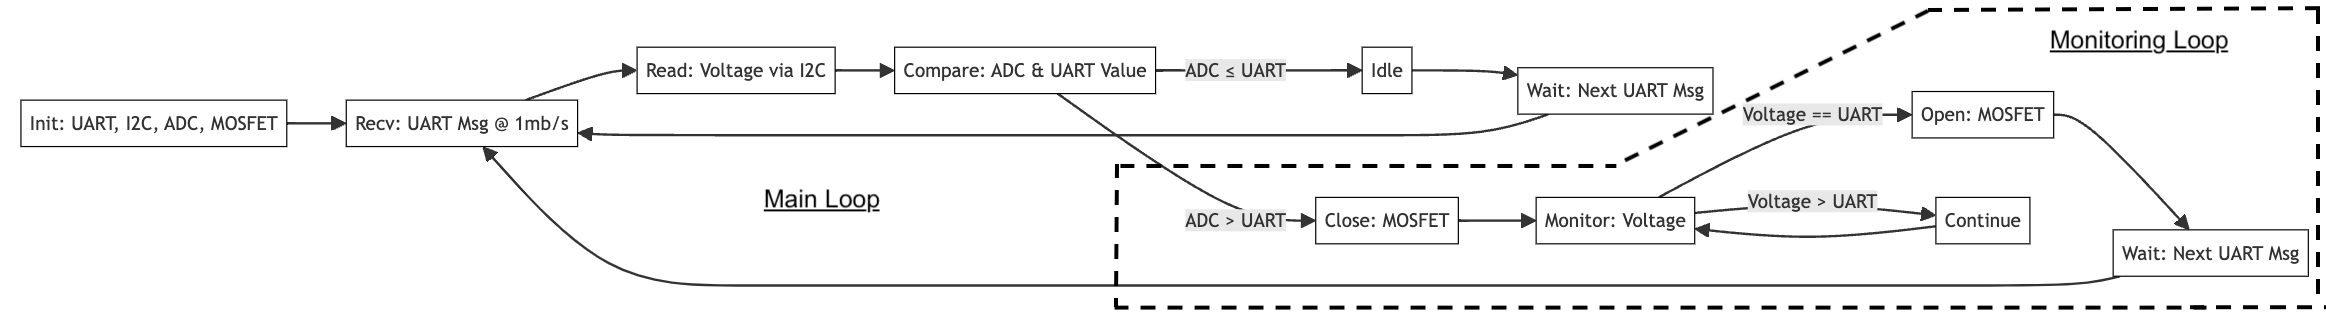
\includegraphics[width=1.0\textwidth]{Skripsie_LaTeXTemplate/Figures/Dumpload_code.png}
\caption{Cell Balancing Test Code Program Flow}
\label{fig:DL_EXP}
\end{figure}
\noindent
The test conducted on the monitoring module affirmed that the system performed in accordance with expectations. The behavior of the system aligned precisely with anticipated outcomes. The ADC provided measurements with a high degree of accuracy, and upon activation, the dump-load circuitry effectively operated at a current of 1A, successfully maintaining the cell voltage at the correct levels throughout the duration of the experiment.\newpage
%*******************************************%
\subsubsection{Controller Current Capability}\label{subsec:Thermal_Test}
%*******************************************%
With assistance from Mr. Petzer, we conducted an experiment using a high-capacity DC power supply and a low-impedance, high-power resistive load. The setup involved connecting the power supply to the main controller board's battery terminals, and the load to the load/charger terminals. The DC isolator successfully separated the power supply side from the load side upon initiation. Engaging the main controller board's relay allowed for a significant 100A current flow. Thermal behavior under these conditions was observed with a Fluke TiS20 thermal camera, as shown in Figure \ref{fig:Thermal}.

\begin{figure}[h!]
\centering
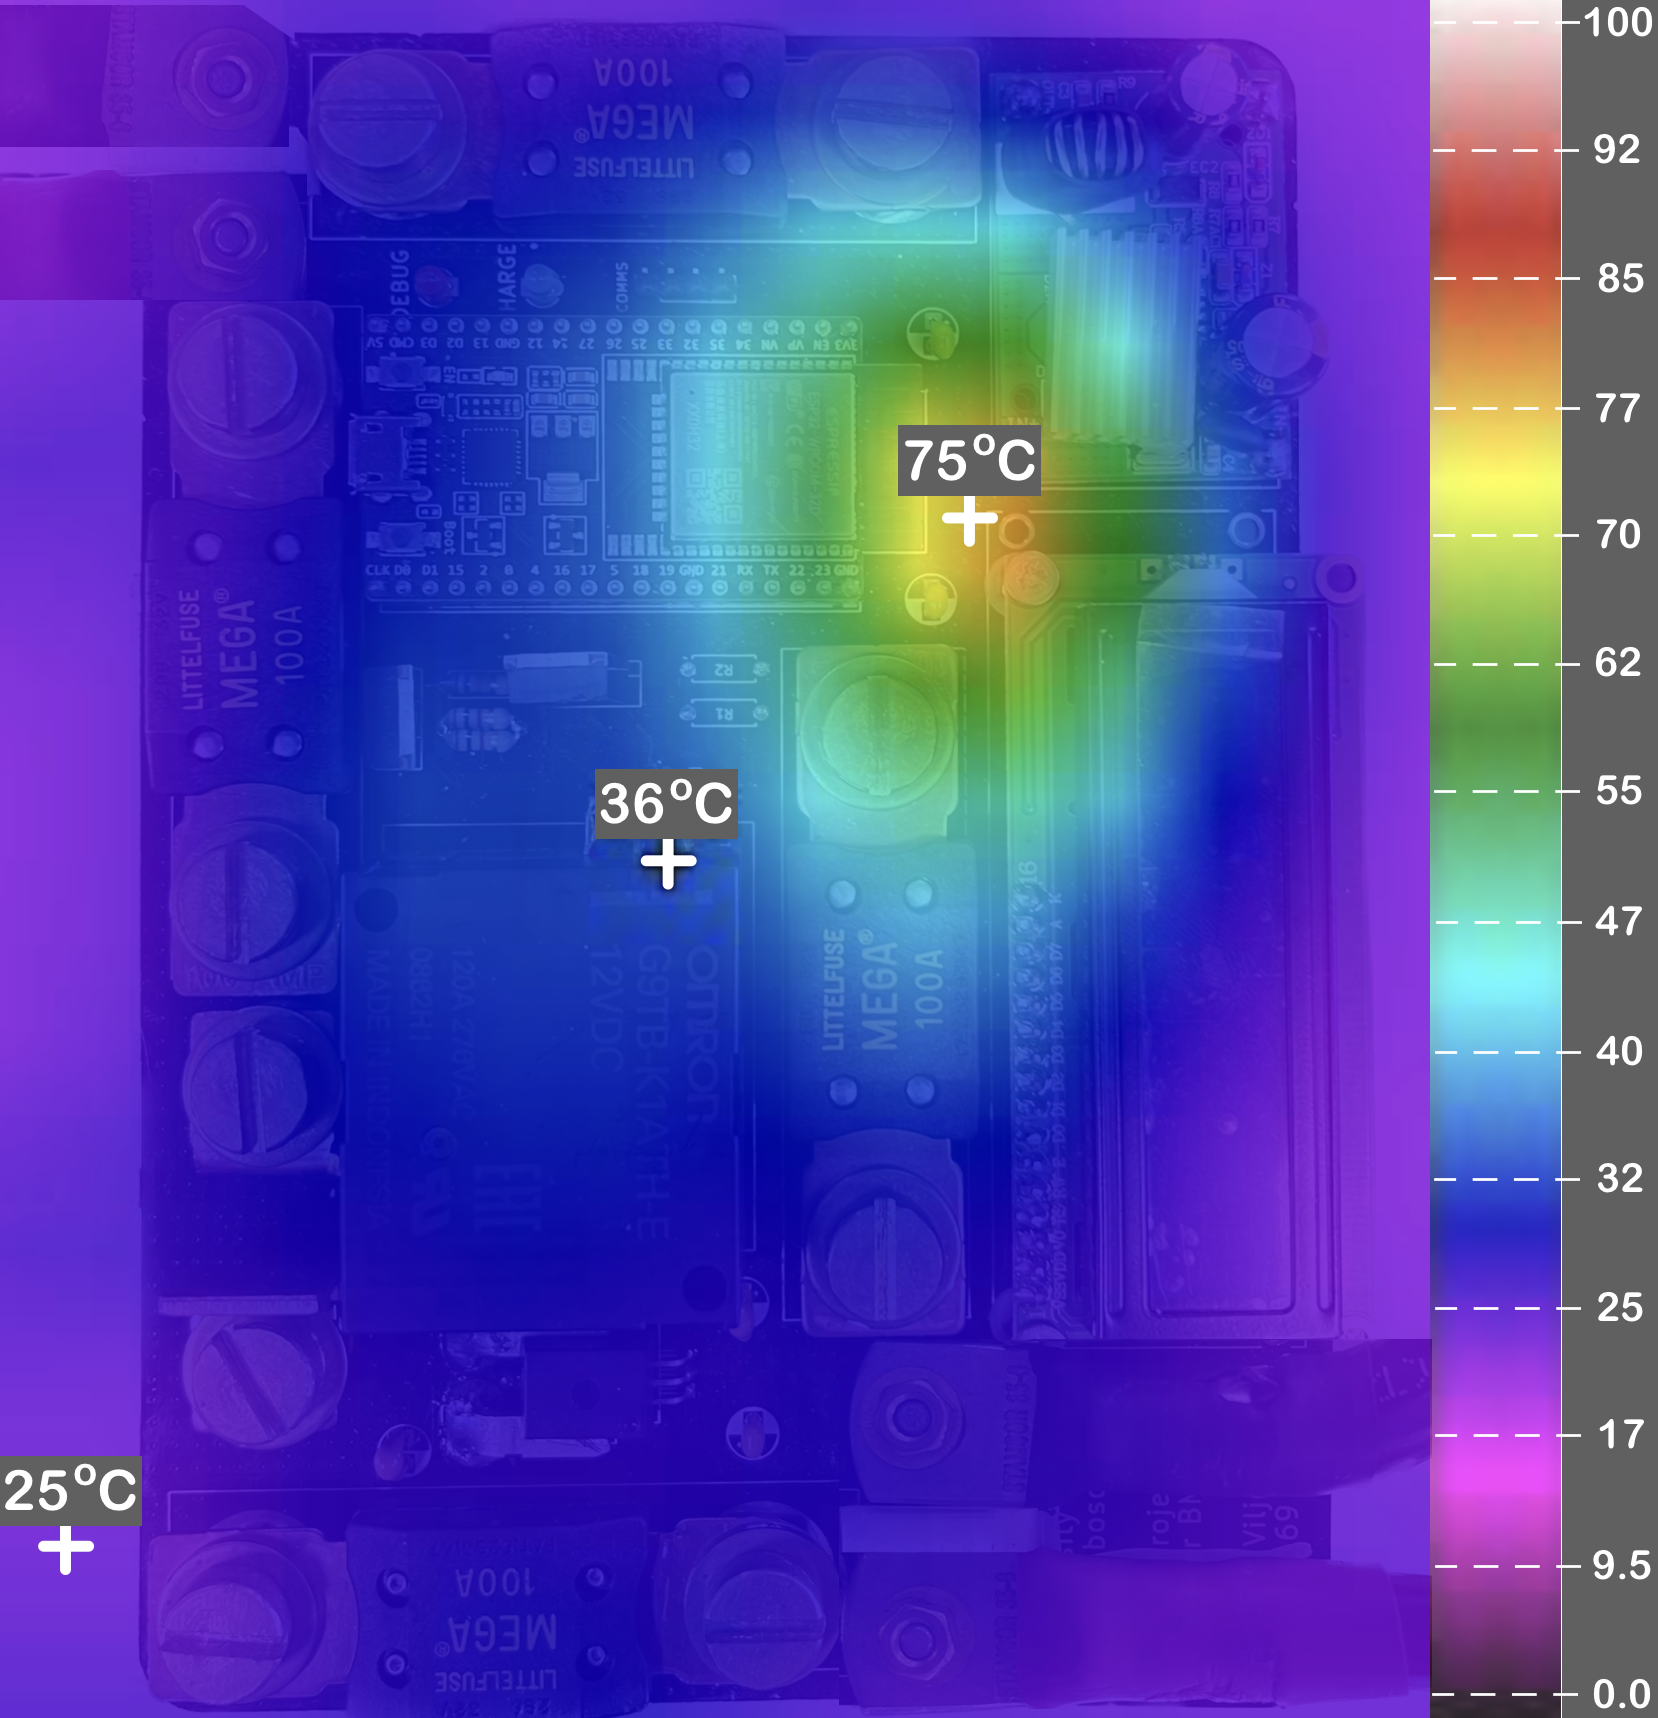
\includegraphics[width=0.4\textwidth]{Figures/thermal_image.png}
\caption{Thermal Imaging with Fluke TiS20}
\label{fig:Thermal}
\end{figure}
\noindent
The thermal image verifies the controller's adequacy in managing the current for both battery and load/charger applications, with a single expected hotspot identified. This hotspot aligns with a known design limitation of the PCB, where a routing constraint for the negative terminal fuses impacted the thermal layout. The current single-sided filled zone with non-connecting vias was a result of this constraint, which was acceptable for the current application. For future enhancements, it is recommended to redesign the PCB to include dual-sided filled zones with via stitching to improve thermal management for high-current operations.
%*******************************************%
\subsubsection{Pulsed Cell Discharge}\label{subsec:pulsemee}
%*******************************************%
The experiment assessed a single 3.2V 100Ah cell's discharge characteristics by connecting it to a $90m\Omega$ load through the main controller, inducing a 35A discharge at 0.33C. The controller executed 17 switch cycles of the DC power relay with a 10-minute pulse width and 25\% duty cycle, to minimize temperature fluctuations and maintain cell stability. Cell voltage and current were meticulously recorded by the monitoring module and logged serially. The collected data was graphically represented to analyze the discharge behavior, as illustrated in Figure \ref{fig:pulsess1}.
\newpage
\begin{figure}[h!]
\centering
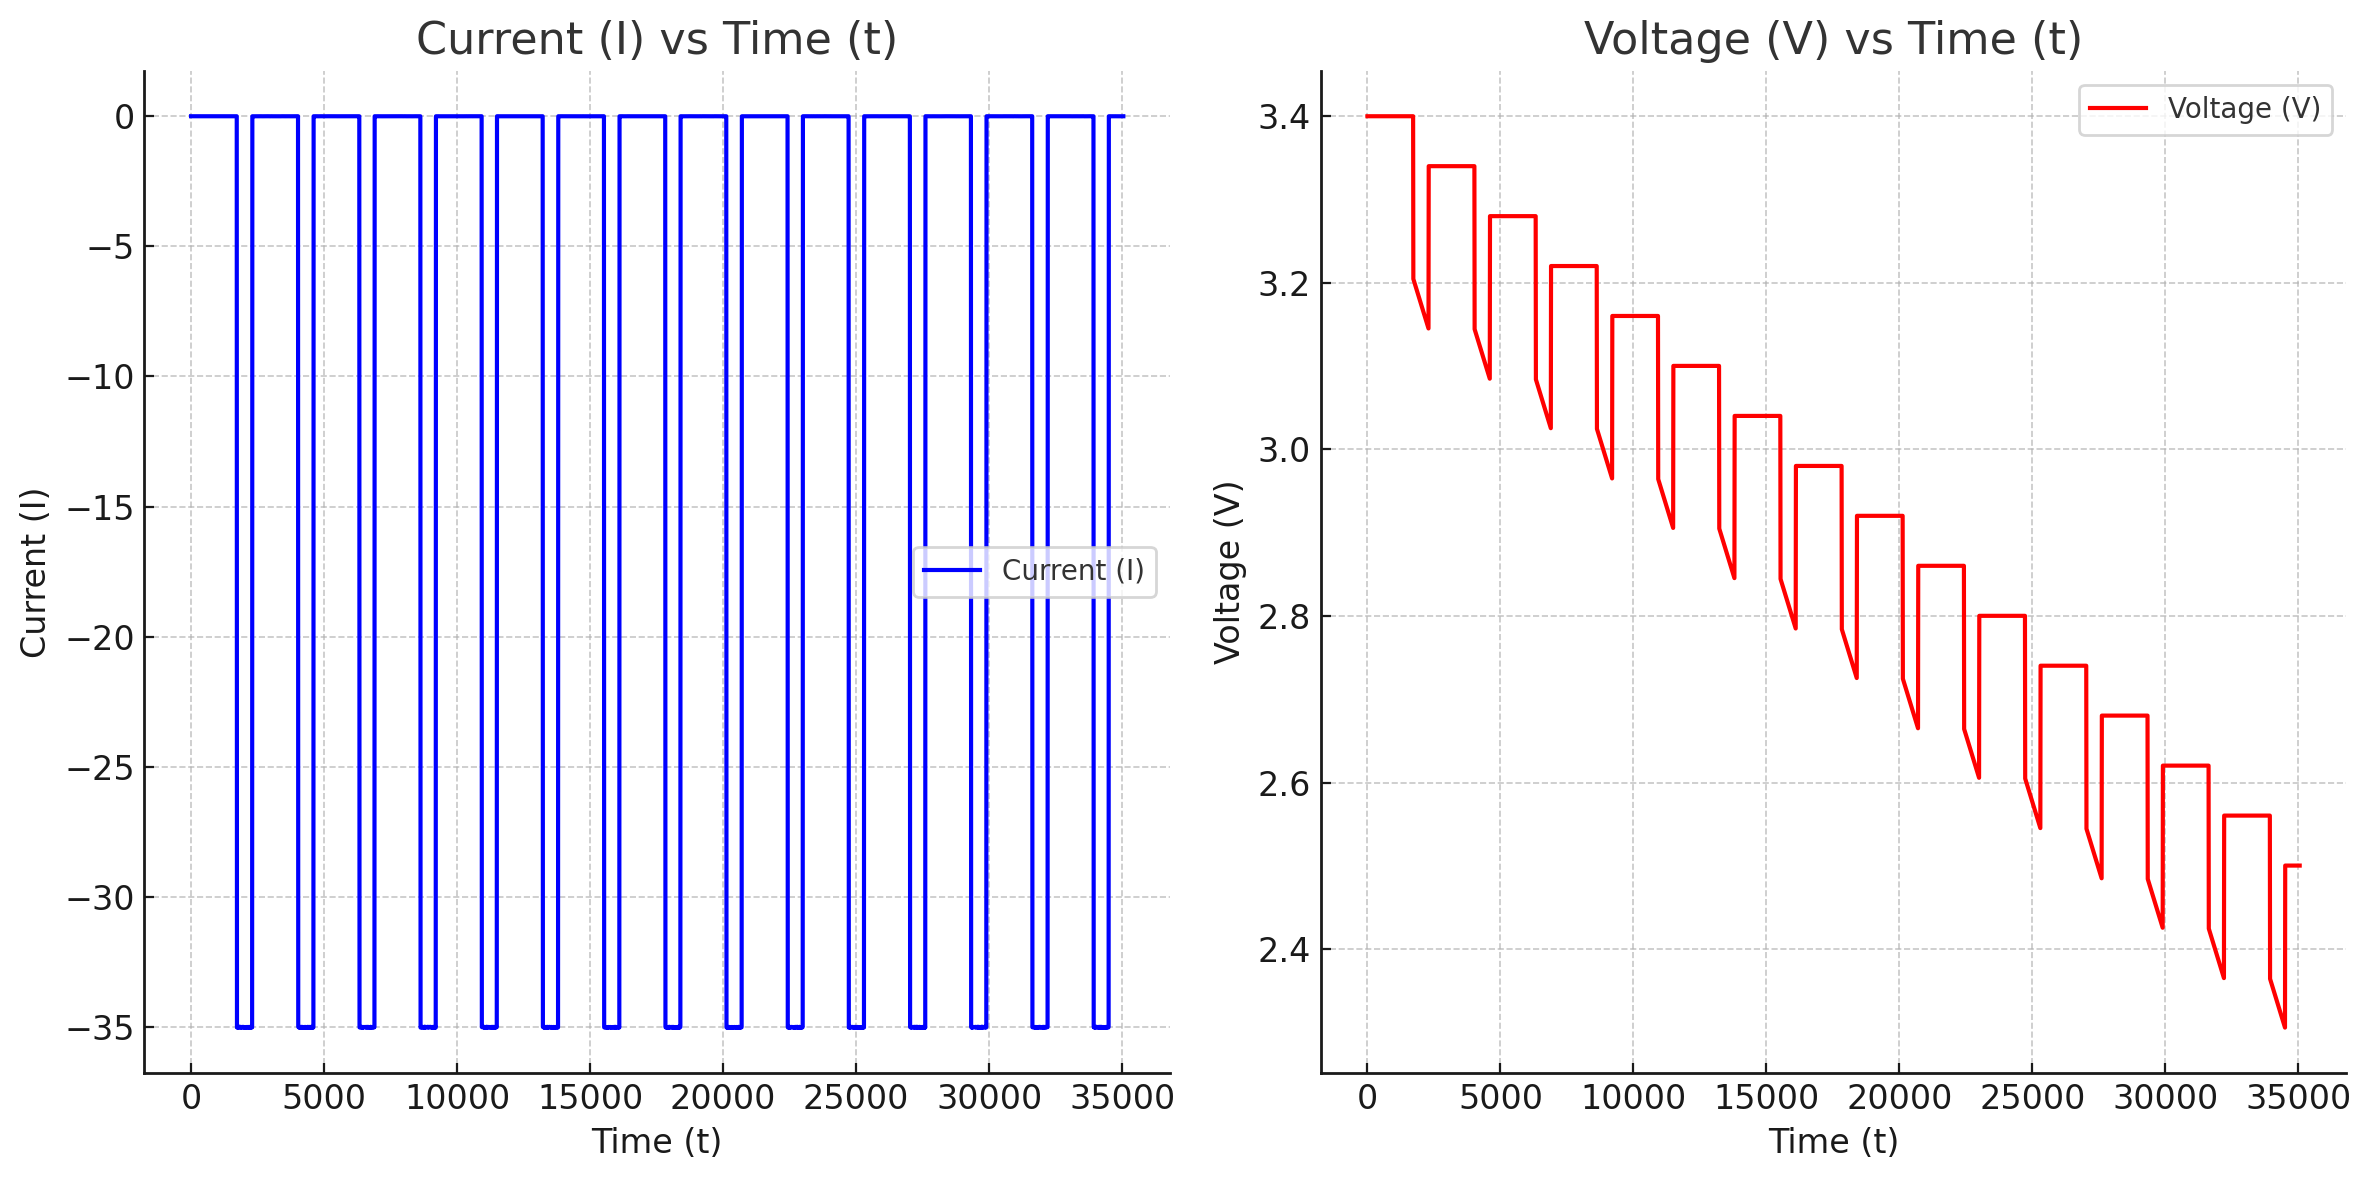
\includegraphics[width=0.6\textwidth]{Skripsie_LaTeXTemplate/Figures/pulseD1.png}
\caption{100Ah 3.2V LFP cell - Pulsed Discharge Current \& Voltage Measured}
\label{fig:pulsess1}
\end{figure}
\noindent
The graphical data from above was imported into MATLAB and analyzed using Javier Gazzarri's battery parameterization model in Simulink \cite{SIMULINKKK}. This facilitated dynamic battery analysis from pulsed discharge data. A modular Battery Management System (BMS) was then developed and simulated in Simulink, utilizing derived parameters to assess system performance. Figure \ref{fig:pulsess2} illustrates the Simulink models and corresponding simulation results. This methodology provided a detailed system evaluation, closely replicating actual battery cell behavior, and confirmed the BMS's operational effectiveness, underscoring Simulink's value in battery system analysis and design.

\begin{figure}[h!]
\centering
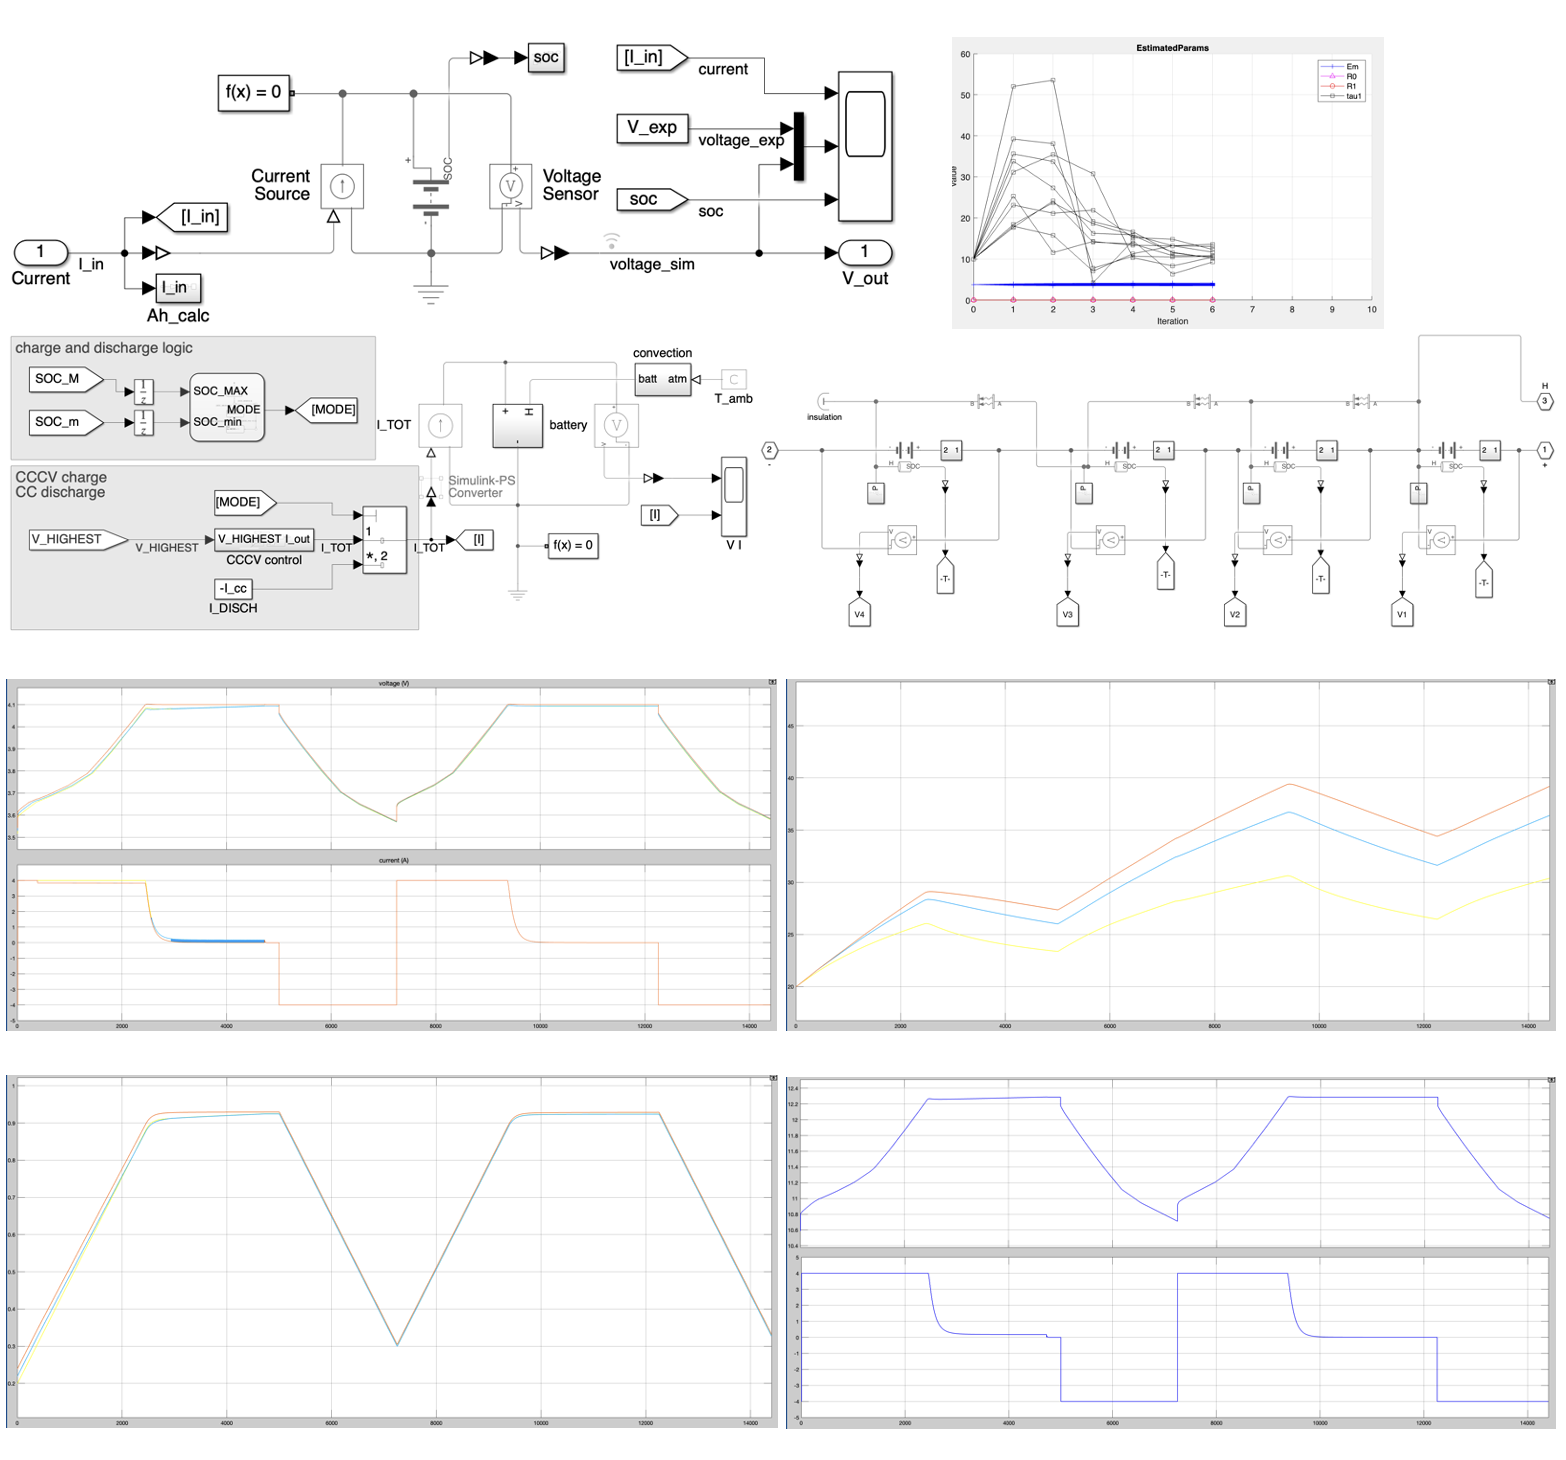
\includegraphics[width=0.8\textwidth]{Skripsie_LaTeXTemplate/Figures/pulseD2.png}
\caption{Simulink Battery Modeling \& Simulated Results \cite{SIMULINKKK}}
\label{fig:pulsess2}
\end{figure}
%*******************************************%


\vfill